%  25 Mar 2026 15:03:52
\documentclass{article}
\usepackage{geometry,booktabs,longtable,pdflscape,rotating,threeparttable,subcaption,graphicx,float}
\usepackage{tabularx,colortbl}
\usepackage[table]{xcolor}
\usepackage{hyperref}
\hypersetup{                           colorlinks=true,                   linkcolor={blue!50!black},                    filecolor={blue!50!black},                 urlcolor={blue!80!black},                     }                              \date{}
\geometry{verbose,letterpaper,lmargin=2.5cm,tmargin=2.5cm}

\begin{document}

\title{Eventstudy Analysis for Displacement Events}
\maketitle
\section{Comparing Eventstudy Specifications}
Next, we compare the eventstudy estimates across different specifications.
\begin{itemize}
\item Raw Means (always good to compare to the eventstudy estimates)
\item OLS - Rel. year effects, no person FE
\item JLS Specification: Cal. year and person FE - since we are not cotrolling for relative year effects, the estimates are not consistent
\item Rel. year effects, person FE
\item Relative year, calendar year and person FE
\item Controlling for fully interacted calendar and relative year effects, as well as person FE
\end{itemize}
\\ The matching design does the heavy lifting, that's why these specification yield very similar results.
\begin{figure}[H] 
\centering 
  \caption{Comparing Eventstudy Specifications} 
\begin{subfigure}{.45\textwidth}
  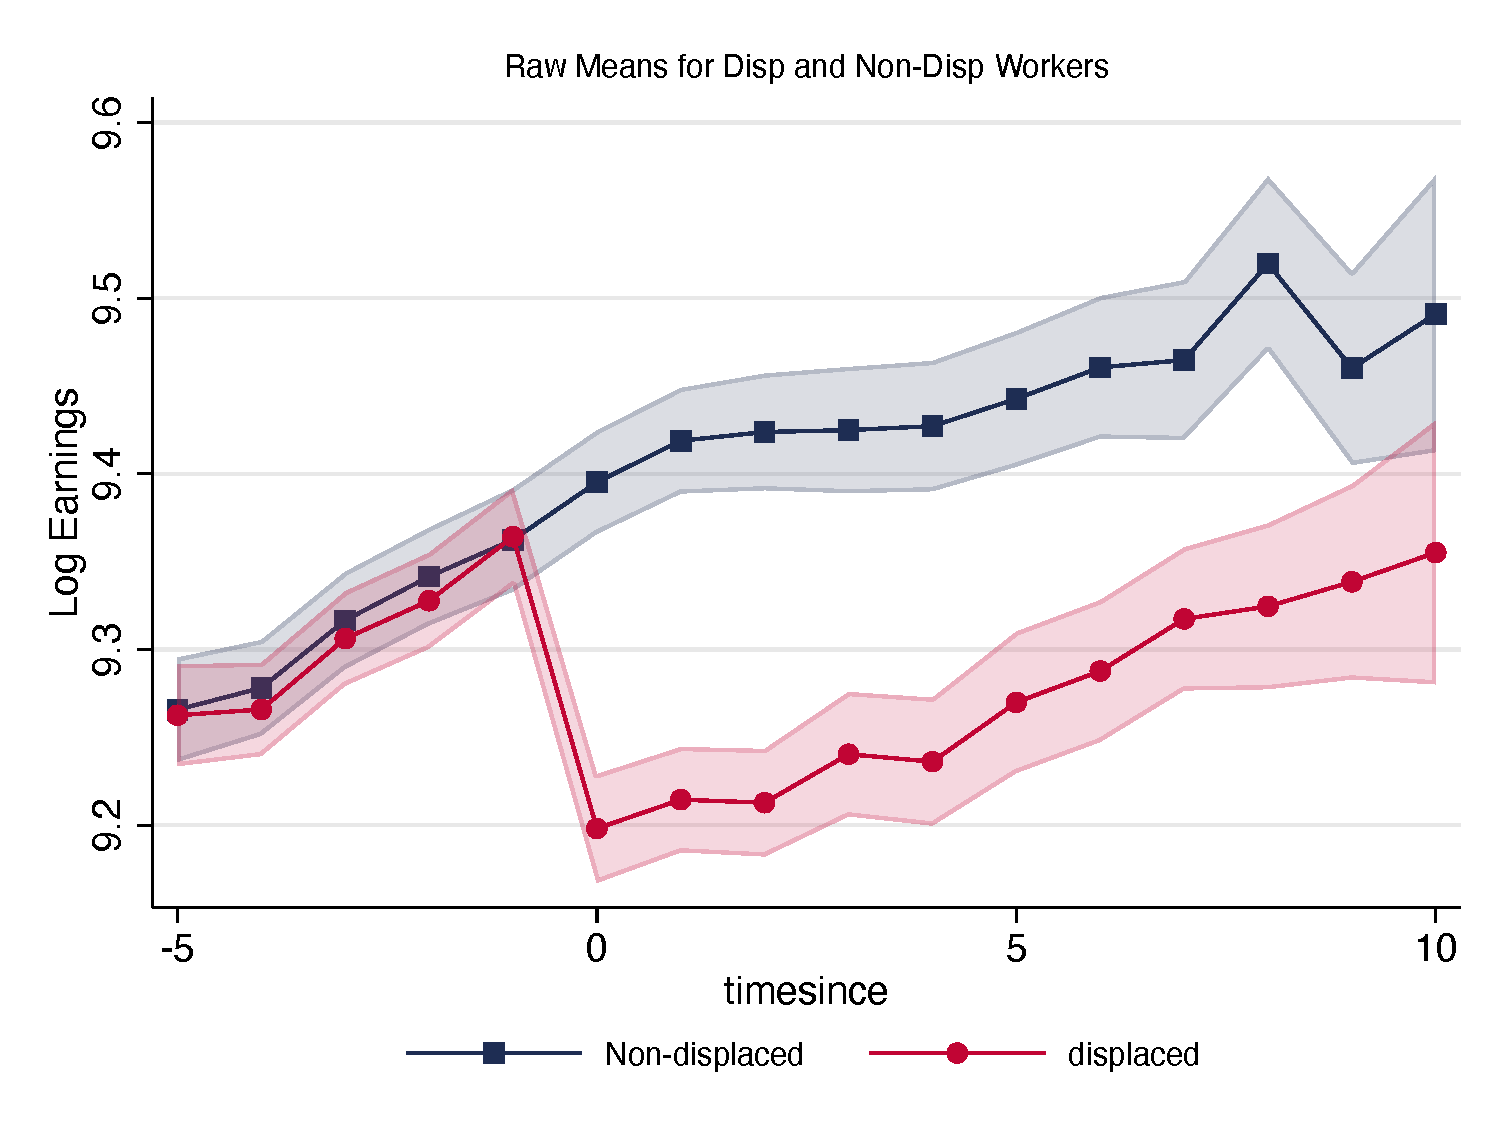
\includegraphics[width = 1.00\textwidth]{Eventstudy/eventstudy_RawMeans.pdf}  
  \caption{Raw Means}
\end{subfigure}
\begin{subfigure}{.45\textwidth}
  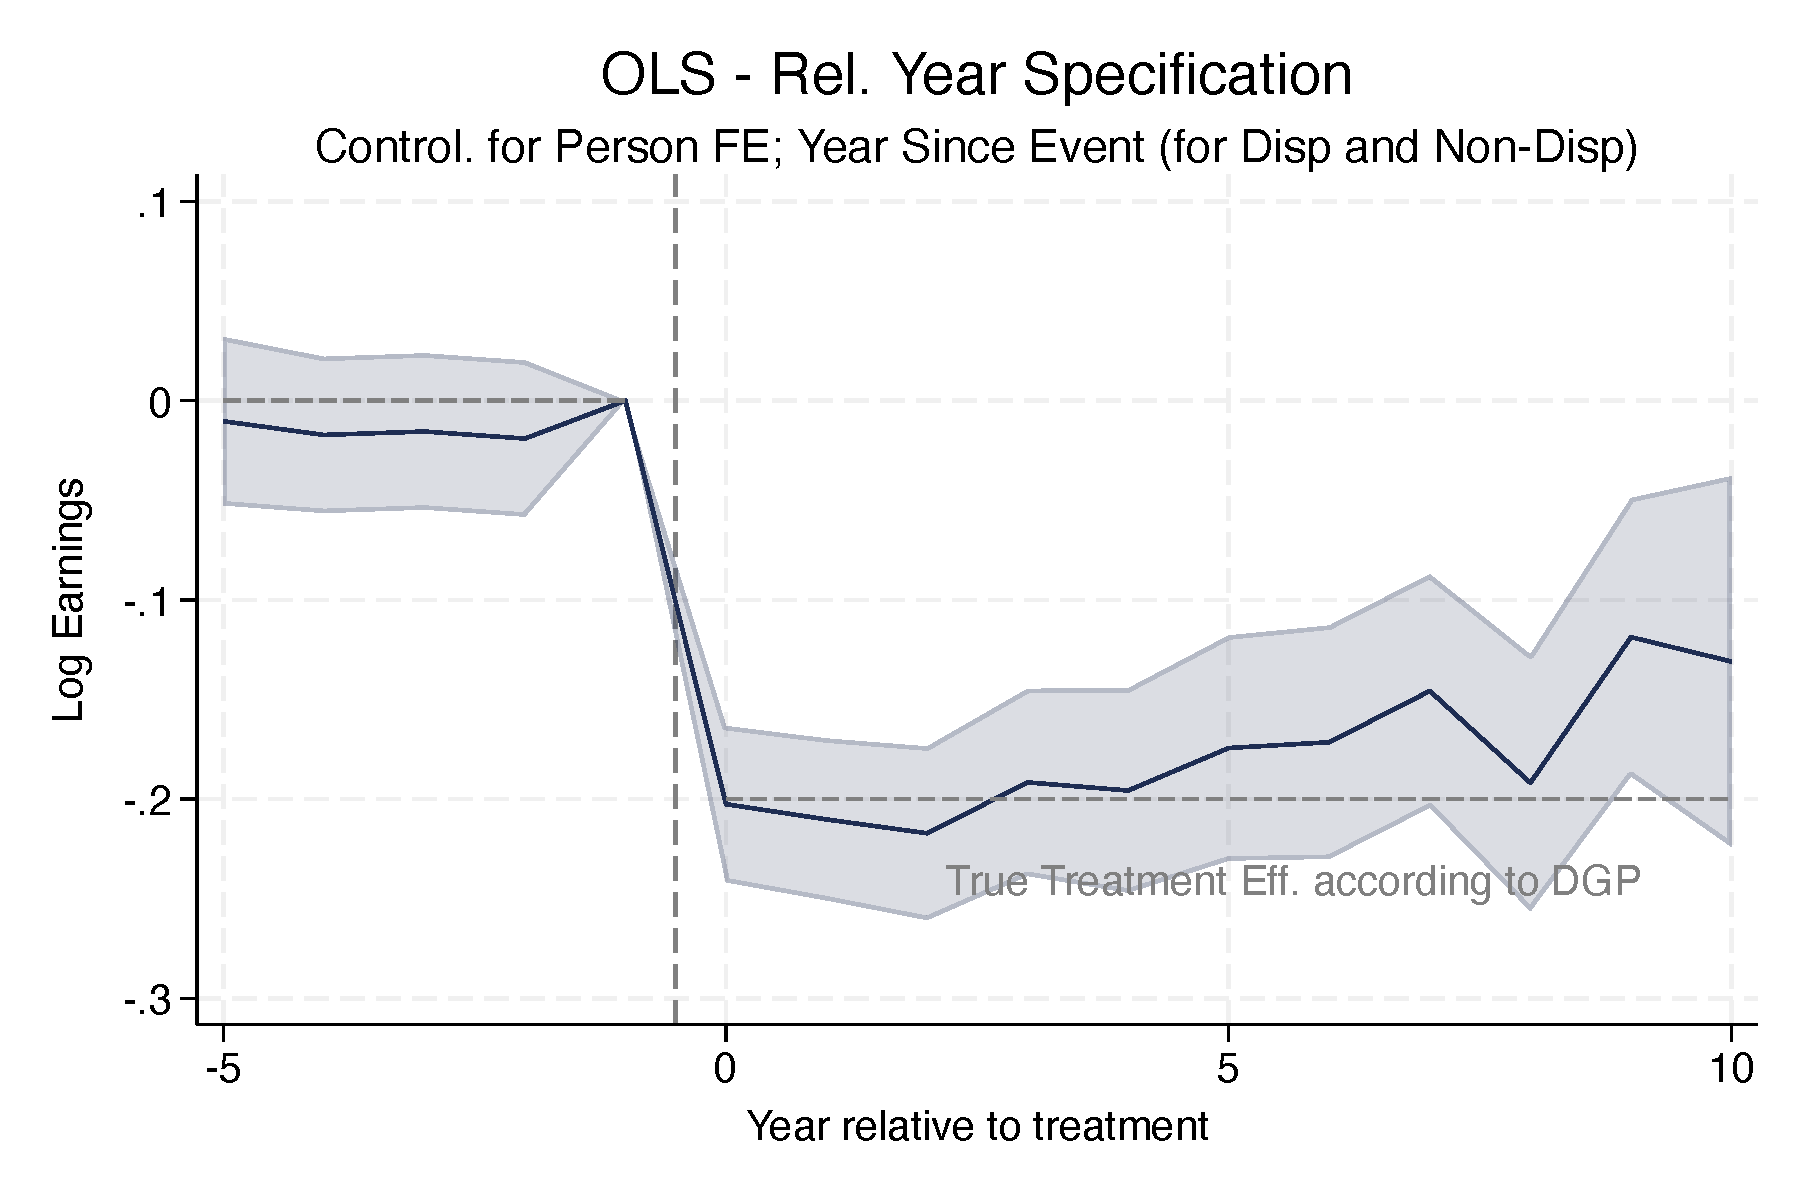
\includegraphics[width = 1.00\textwidth]{Eventstudy/eventstudy_OLS.pdf}  
  \caption{Rel. year effects, no person FE}
\end{subfigure}
\begin{subfigure}{.45\textwidth}
  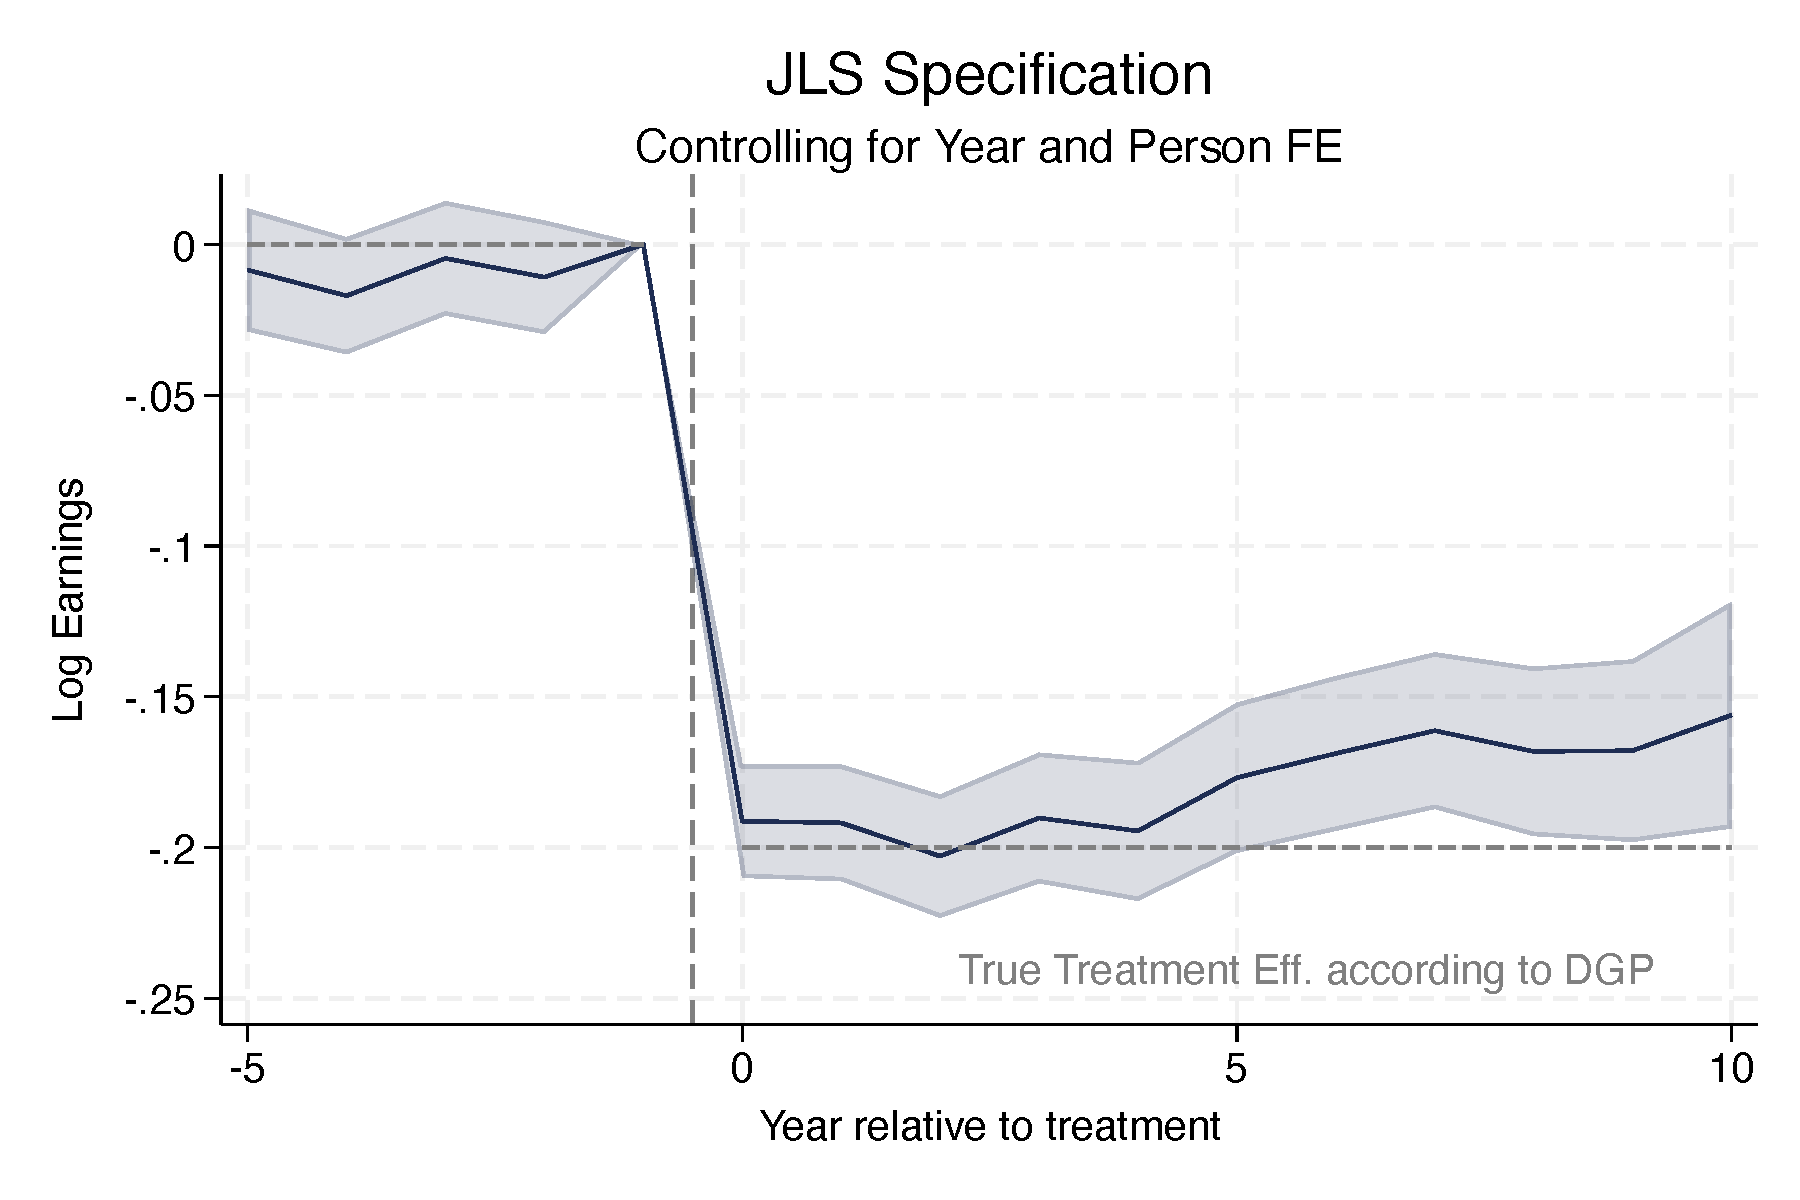
\includegraphics[width = 1.00\textwidth]{Eventstudy/eventstudy_FE_JLS.pdf}  
  \caption{Cal. year and person FE - does not work!}
\end{subfigure}
\begin{subfigure}{.45\textwidth}
  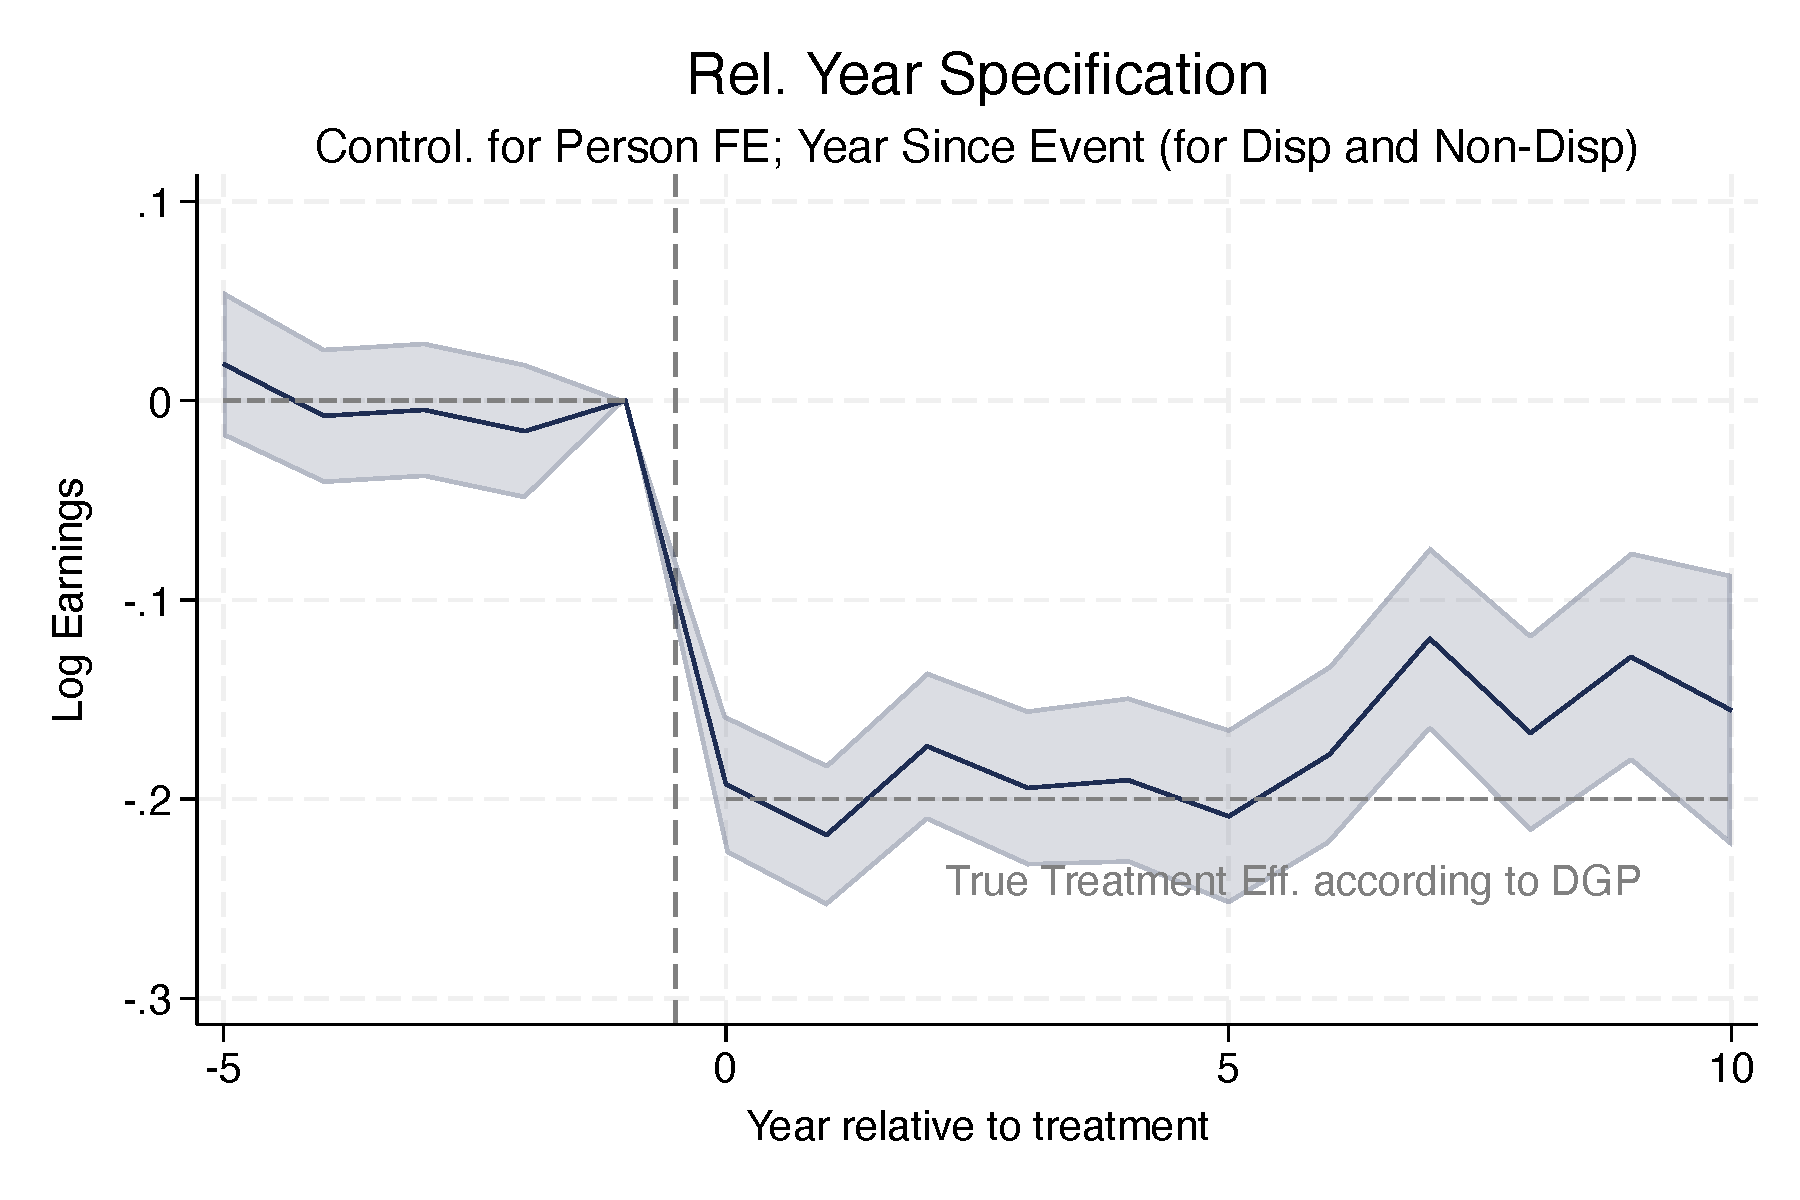
\includegraphics[width = 1.00\textwidth]{Eventstudy/eventstudy_FE_RelYear.pdf}  
  \caption{Rel. year effects, person FE}
\end{subfigure}
\begin{subfigure}{.45\textwidth}
  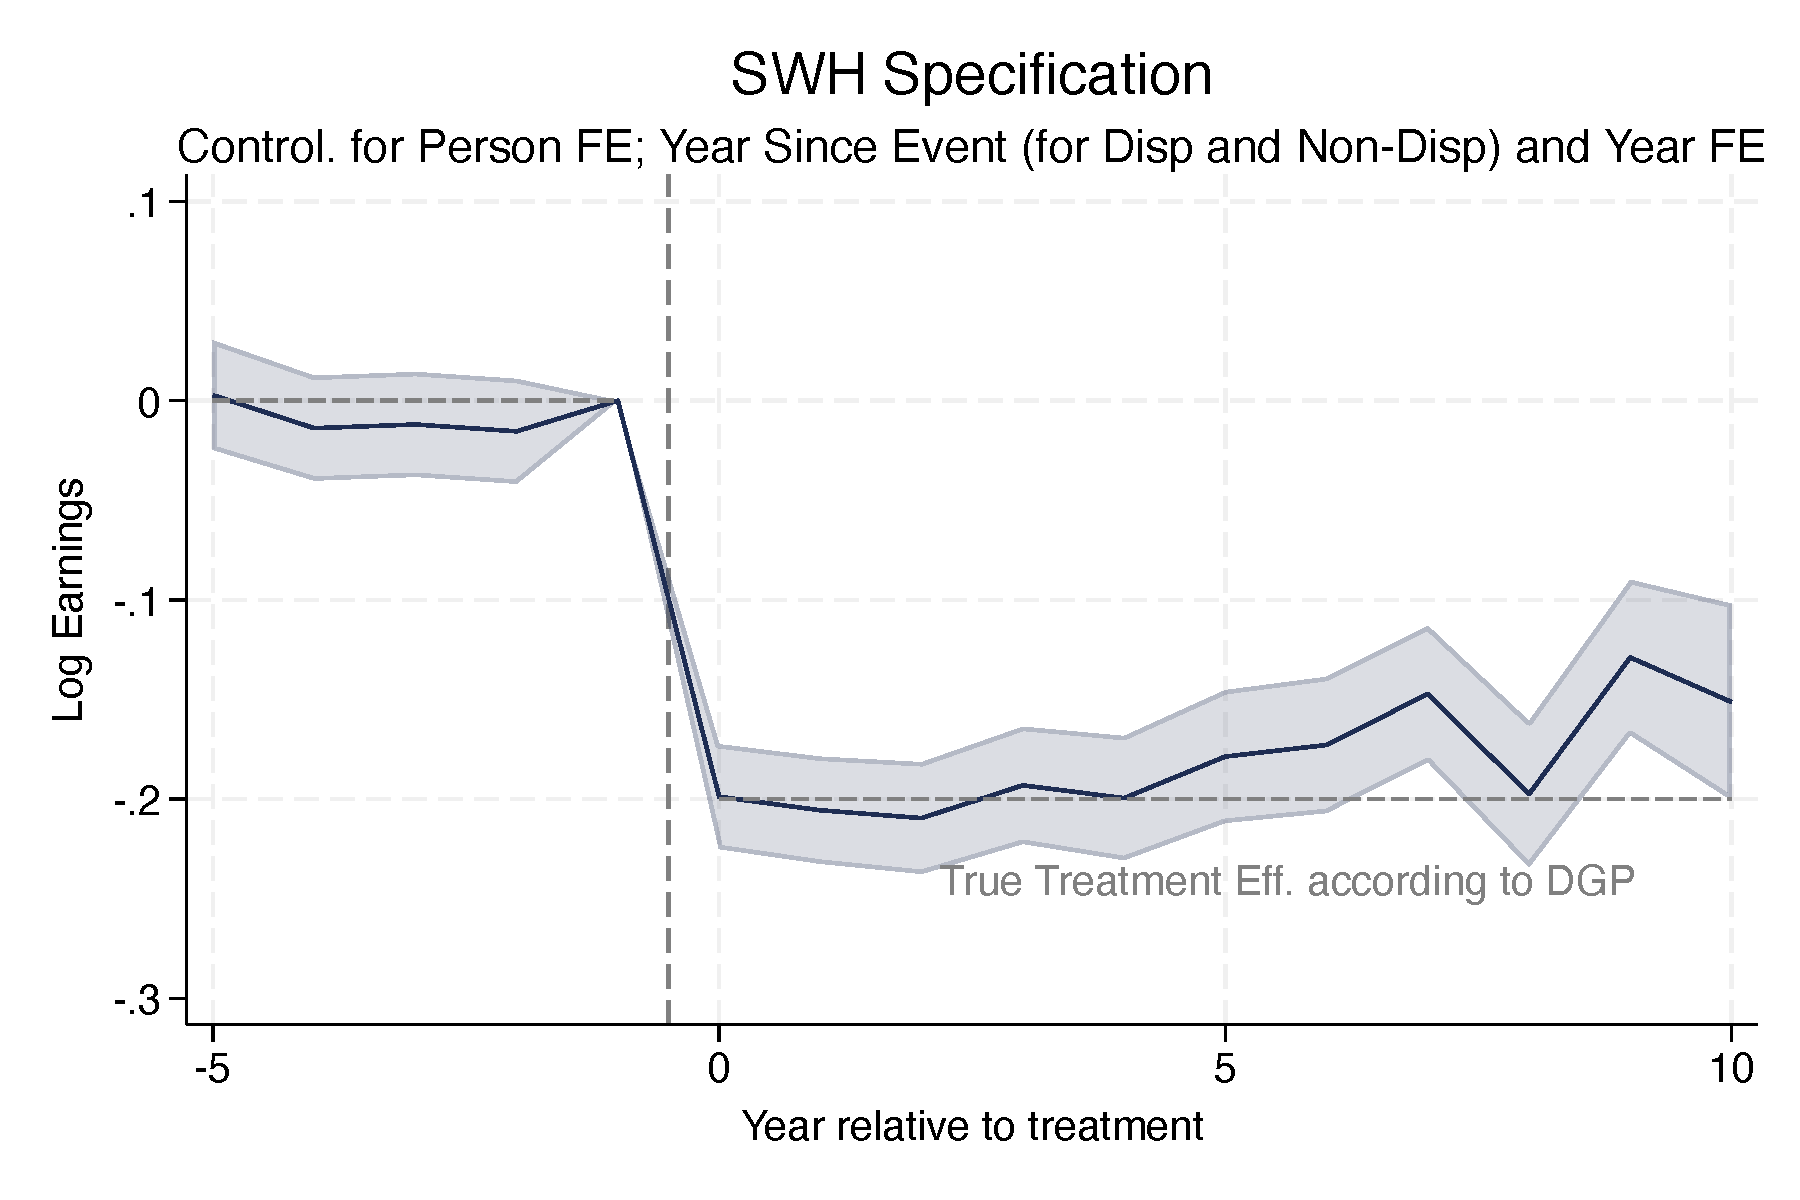
\includegraphics[width = 1.00\textwidth]{Eventstudy/eventstudy_FE_Full.pdf}  
  \caption{Rel. year, cal. year and person FE}
\end{subfigure}
\begin{subfigure}{.45\textwidth}
  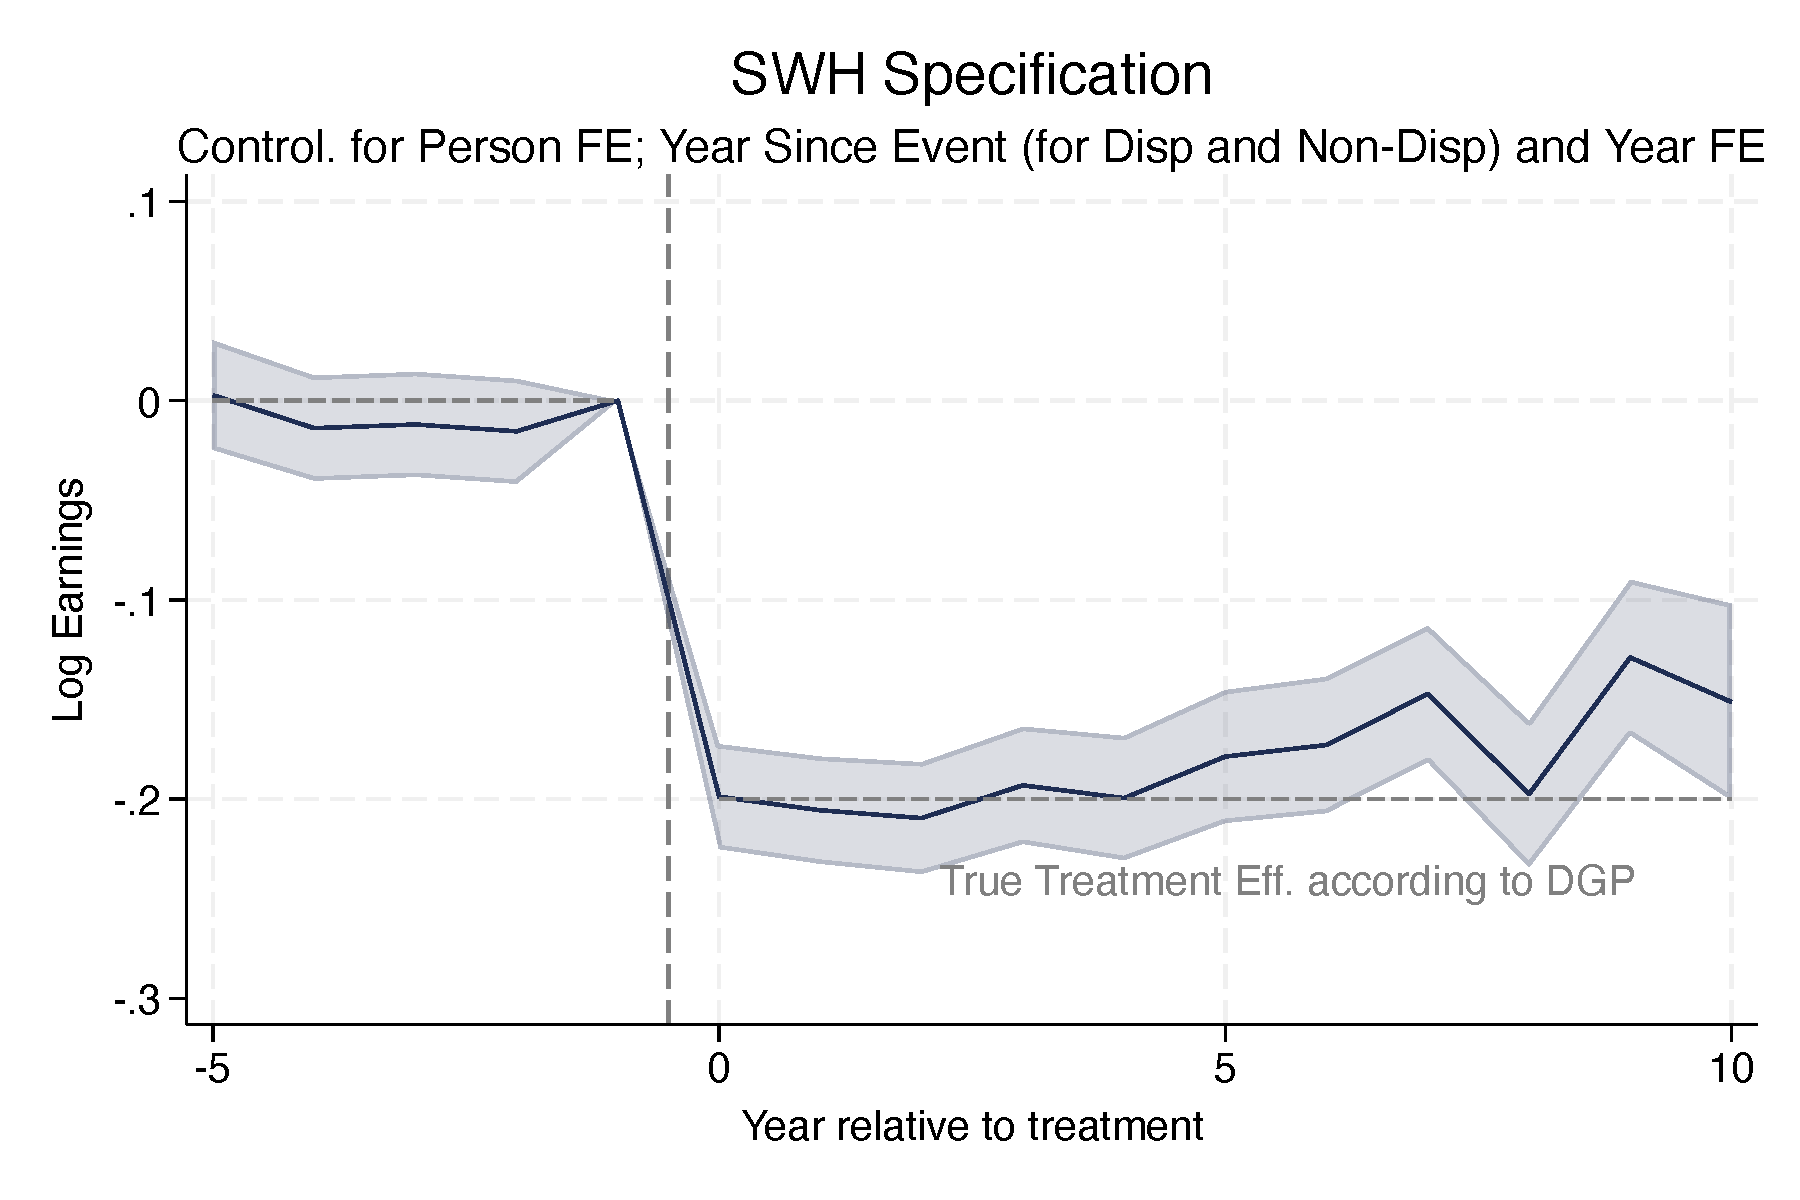
\includegraphics[width = 1.00\textwidth]{Eventstudy/eventstudy_FE_Full.pdf}  
  \caption{Rel. year $\times$ cal. year and person FE}
\end{subfigure}
\end{figure} 
\clearpage \newpage
\section{Different Outcomes}
Next, we create eventstudy estimates for different outcomes.
\begin{itemize}
\item Earnings in Levels
\item Earnings Growth
\item Log Earnings conditional on positive earnings
\item Employment
\end{itemize}
\begin{figure}[H] 
\centering 
  \caption{Event Study Estimates for Different Outcomes} 
\begin{subfigure}{.45\textwidth}
  \includegraphics[width = 1.00\textwidth]{Eventstudy/eventstudy_earn.pdf}  
  \caption{Earnings in Levels}
\end{subfigure}
\begin{subfigure}{.45\textwidth}
  \includegraphics[width = 1.00\textwidth]{Eventstudy/eventstudy_employed.pdf}  
  \caption{Employment}
\end{subfigure}
\begin{subfigure}{.45\textwidth}
  \includegraphics[width = 1.00\textwidth]{Eventstudy/eventstudy_logearn.pdf}  
  \caption{Log Earnings cond. on pos. Earnings}
\end{subfigure}
\begin{subfigure}{.45\textwidth}
  \includegraphics[width = 1.00\textwidth]{Eventstudy/eventstudy_earnings_growth.pdf}  
  \caption{Earnings Growth}
\end{subfigure}
\end{figure} 
\clearpage \newpage
\section{Different Outcomes}
Next, we create eventstudy estimates for different outcomes.
\begin{itemize}
\item Scale Raw Mean Difference by Control Mean: 
\begin{itemize}
\item Outcome: $\frac{\bar{y}_{t}^{D} - \bar{y}_{t}^{ND}}{\bar{y}_{t}^{ND}}$
\end{itemize}
\item Scale Regression Coefficient from level regression by Control Mean: 
\begin{itemize}
\item Outcome: $ y_{it}$
\item Regression: $ y_{it} = \alpha_i + \gamma_t + \sum_k \beta_k D_{it}^k + \varepsilon_{it}$
\item Scale: $\frac{\hat{\beta}_t}{E[y_{it}|X_{it},Non-Displaced]}$
\end{itemize}
\item Poisson QMLE: 
\begin{itemize}
\item Outcome: {it}$ (same as Approaches 1 and 2)
\item Regression model: $ E[y_{it}|X_{it}] = \exp(\alpha_i + \gamma_t + \sum_k \beta_k D_{it}^k), $
\item Scale: $\exp(\hat{\beta}_t) - 1$
\end{itemize}
\item Earnings Growth in percent: 
\begin{itemize}
\item Outcome: $ \Delta y_{i,t} = \frac{y_{i,t} - y_{i,-1}}{y_{i,-1}}$
\item Regression: $ \Delta y_{i,t} = \alpha_i + \gamma_t + \sum_k \beta_k D_{it}^k + \varepsilon_{it}$
\item Scale: $\beta_t$
\end{itemize}
\subsection*{Discussion: Comparing Approaches for Percentage Interpretation}
Each of these approaches expresses earnings losses as a percentage, but they differ in their
assumptions, what they estimate, and how they handle zero earnings.
\\
\textbf{Scaling by the control group mean (Approaches 1 and 2).}
With a matching design, the control group mean is a valid estimate of the counterfactual
$ E[Y(0)|D=1]$, so dividing the treatment--control difference by the control mean yields a proper
estimate of the ATT in percentage terms: $\text{ATT} / E[Y(0)|D=1]$.
Approach 1 (raw mean difference) is fully nonparametric---transparent and easy to compute.
Approach 2 adds person fixed effects and controls, which may improve precision and absorb
remaining imbalance after matching, but should yield similar point estimates if matching quality
is high. Both approaches handle zero earnings naturally since they operate in levels.
A minor disadvantage is that confidence intervals from dividing $\hat{\beta}_t$ by $\bar{y}_t^{ND}$
are approximate---strictly, one would need the delta method or bootstrap to account for
estimation error in the denominator.
This is the classic approach used in the job displacement literature
(Jacobson, LaLonde, and Sullivan, 1993, \textit{AER}).
\\
\textbf{Poisson QMLE (Approach 3).}
Like Approaches 1 and 2, Poisson QMLE uses earnings in levels $ y_{it}$ as the outcome
and estimates essentially the same parameter---the percentage treatment effect---but
does so directly via the multiplicative model
$ E[y_{it}|X] = \exp(\alpha_i + \gamma_t + \sum_k \beta_k D_{it}^k)$,
so $\exp(\hat{\beta}_t) - 1$ gives the percentage effect without requiring post-estimation rescaling.
Key properties:
\begin{itemize}
\item \textit{Handles zeros naturally:} Unlike $\log(y)$, Poisson PML is well-defined for $ y=0$
since it only requires correct specification of the conditional mean, not that $ y$ follows
a Poisson distribution (Santos Silva and Tenreyro, 2006, \textit{REStat};
Gourieroux, Monfort, and Trognon, 1984, \textit{Econometrica}).
High-dimensional fixed effects can be included via \texttt{ppmlhdfe}
(Correia, Guimar\~{a}es, and Zylkin, 2020, \textit{Stata Journal}).
\item \textit{Functional form difference vs.\ OLS:}
OLS in levels assumes \textbf{additive separability}:
$ E[y|i,t,D] = \alpha_i + \gamma_t + \beta D$---the treatment effect is the same
\textit{absolute} amount for everyone.
Poisson assumes \textbf{multiplicative separability}:
$ E[y|i,t,D] = \exp(\alpha_i) \cdot \exp(\gamma_t) \cdot \exp(\beta D)$---the treatment
effect is the same \textit{proportional} amount for everyone.
When the goal is a percentage interpretation, the multiplicative assumption is arguably
more natural: a 20\% earnings loss means higher-earning workers lose more in levels,
which is typically what we observe empirically.
\item \textit{Same estimand as Approaches 1 and 2:}
With few controls, $\exp(\hat{\beta}^{\text{Poisson}}_t) - 1 \approx \hat{\beta}^{\text{OLS}}_t / \bar{y}$,
so all three approaches estimate essentially the same percentage effect.
Differences emerge when effects are large or when the outcome distribution has many zeros.
\end{itemize}
\\
\textbf{Earnings growth (Approach 4).}
This measures the individual-level percentage change $(y_{it} - y_{i,-1}) / y_{i,-1}$,
which is directly interpretable at the individual level. However, it is \textit{undefined}
when baseline earnings are zero, so it drops the extensive margin entirely.
It can also be extremely noisy or ill-behaved when the denominator is small.
This is a serious limitation whenever non-employment spells are prevalent.
\\
\textbf{Summary.}
When zeros are rare (as for main worker earnings before displacement), all four approaches
should yield similar results. Differences emerge when zeros are prevalent---precisely
the case for spousal outcomes and the added worker effect.
\begin{figure}[H] 
\centering 
  \caption{Expressing Earnings Losses in Percent (incl. zero earnings)} 
\begin{subfigure}{.45\textwidth}
  \includegraphics[width = 1.00\textwidth]{Eventstudy/eventstudy_mean_diff.pdf}  
  \caption{Scale Raw Mean Difference: $\frac{\bar{y}_{t}^{D} - \bar{y}_{t}^{ND}}{\bar{y}_{t}^{ND}}$}
\end{subfigure}
\begin{subfigure}{.45\textwidth}
  \includegraphics[width = 1.00\textwidth]{Eventstudy/eventstudy_pct_control.pdf}  
  \caption{Scale Regression Coefficient: $\frac{\hat{\beta}_t}{\bar{y}_{t}^{ND}}$}
\end{subfigure}
\begin{subfigure}{.45\textwidth}
  \includegraphics[width = 1.00\textwidth]{Eventstudy/eventstudy_poisson_pct.pdf}  
  \caption{Poisson QMLE, scaled to \%: $\exp(\hat{\beta}_t) - 1$}
\end{subfigure}
\begin{subfigure}{.45\textwidth}
  \includegraphics[width = 1.00\textwidth]{Eventstudy/eventstudy_earnings_growth.pdf}  
  \caption{Earnings Growth: $\frac{y_{i,t} - y_{i,-1}}{y_{i,-1}}$}
\end{subfigure}
\end{figure} 
\clearpage \newpage
\section{Added Worker Effect: Spousal Outcomes}
This section estimates the \textbf{added worker effect} (AWE) --- the change in spousal labor market outcomes
in response to the primary worker's job displacement.
\\ We estimate event study regressions using the same treatment x relative-time dummies
as for the main worker outcomes, but with spouse earnings, employment, and various transformations as dependent variables.
\\
\textbf{Note on zero baseline earnings:} About 40\% of spouses have zero earnings at baseline.
This makes expressing the AWE in percentage terms considerably more challenging than for the
displaced worker's own earnings.
\\
We present the following approaches:
\begin{itemize}
\item \textbf{Levels and Employment} (panels a--d): Raw means and event study estimates for
spouse earnings in levels and employment. Well-defined for all observations.
\item \textbf{Scale by Control Mean} (panels e--f): Raw mean difference and regression coefficient
divided by the control group mean at each event time.
\item \textbf{Poisson QMLE} (panel g): $ \exp(\hat{\beta}_t) - 1$ handles zeros naturally.
\item \textbf{Earnings Growth as \% of HH Income} (panel h): $ (y_{it}^S - y_{i,-1}^S) / (y_{i,-1} + y_{i,-1}^S)$.
\item \textbf{Earnings Growth as \% of Partner Earnings} (panel i): $ (y_{it}^S - y_{i,-1}^S) / y_{i,-1}$.
\item \textbf{Log with additive constant} (panels j--l): $ \log(y^S + c)$ for $ c \in \{0.01, 1, 100\}$.
\end{itemize}
\subsection*{Discussion: Percentage Interpretation for the Added Worker Effect}
\textbf{The zero-baseline problem.}
Earnings growth $ (y_{it}^S - y_{i,-1}^S) / y_{i,-1}^S$ is undefined when baseline spouse
earnings are zero. Conditioning on positive baseline earnings creates a selected sample:
the extensive margin response---spouses \textit{entering} the labor force in response to
displacement---is missed entirely, even though it may be an important component
of the AWE (Lundberg, 1985, \textit{JPE}; Stephens, 2002, \textit{JLE}).
\textbf{Dividing by spouse baseline income does not work} for the full sample since it
drops the approximately 40\% of spouses who are not employed at baseline.
\\
\textbf{Scaling by the control mean.}
Dividing the level estimate by the control group mean works and includes all observations
(zeros contribute to both numerator and denominator). However, when the control mean is
small---as it is for initially non-employed spouses---small level changes can produce
large and potentially misleading percentages.
\\
\textbf{Poisson QMLE targets the same parameter as scaling by the control mean.}
Like Approaches 1 and 2, Poisson QMLE uses spouse earnings in levels $ y_{it}^S$ as the outcome.
With few controls, $ \exp(\hat{\beta}^{\text{Poisson}}_t) - 1 \approx \hat{\beta}^{\text{OLS}}_t / \bar{y}^S$,
so all three approaches estimate essentially the same percentage effect.
The advantage of Poisson is that it handles zeros without any sample restriction or ad-hoc rescaling,
gives a coherent percentage interpretation via $ \exp(\hat{\beta}_t) - 1$, and captures both extensive and
intensive margin responses in a single estimate. The multiplicative structure is especially
appropriate here: when baseline spouse earnings are zero, the model implies zero expected
contribution from the intensive margin, which is correct.
\\
\textbf{Earnings growth relative to household income.}
Normalizing by total household baseline earnings
$ (y_{i,-1} + y_{i,-1}^S)$ instead of spouse baseline earnings alone
is always defined (since the primary worker has positive earnings by construction)
and has a natural interpretation: it measures the spousal earnings response as a share of
total household resources at risk.
\\
\textbf{Earnings growth relative to partner (displaced worker) income.}
Normalizing by the displaced worker's baseline earnings $ y_{i,-1}$ uses the same
denominator as the displaced worker's own earnings growth measure
$ (y_{it} - y_{i,-1})/y_{i,-1}$.
This makes the two directly additive: the displaced worker's earnings growth
plus the spouse's earnings growth (both normalized by the displaced worker's
pre-displacement earnings) gives the total household income change as a fraction
of the displaced worker's baseline earnings.
This is always well-defined since displaced workers have positive baseline earnings by construction.
\\
\textbf{Log transformation with additive constant: $ \log(y^S + c)$.}
A common approach to handle zero earnings is to estimate $ \log(y + c)$ for some
constant $ c > 0$. However, Chen and Roth (\textit{QJE}, 2024) show that the
estimated treatment effect is highly sensitive to the choice of $ c$ and that
there is no principled way to select it.
We illustrate this with $ c \in \{0.01, 1, 100\}$.
The results vary dramatically across choices of $ c$, confirming that this approach
is unreliable for outcomes with many zeros.
\begin{figure}[H] 
\centering 
  \caption{Added Worker Effect: All Spouses} 
\begin{subfigure}{.24\textwidth}
  \includegraphics[width = 1.00\textwidth]{Spouse_eventstudy/eventstudy_spouse_earn_RawMeans_all.pdf}  
  \caption{Raw Means: Earnings}
\end{subfigure}
\begin{subfigure}{.24\textwidth}
  \includegraphics[width = 1.00\textwidth]{Spouse_eventstudy/eventstudy_spouse_employed_RawMeans_all.pdf}  
  \caption{Raw Means: Employment}
\end{subfigure}
\begin{subfigure}{.24\textwidth}
  \includegraphics[width = 1.00\textwidth]{Spouse_eventstudy/eventstudy_spouse_earn_all.pdf}  
  \caption{Event Study: Earnings}
\end{subfigure}
\begin{subfigure}{.24\textwidth}
  \includegraphics[width = 1.00\textwidth]{Spouse_eventstudy/eventstudy_spouse_employed_all.pdf}  
  \caption{Event Study: Employment}
\end{subfigure}
\begin{subfigure}{.24\textwidth}
  \includegraphics[width = 1.00\textwidth]{Spouse_eventstudy/eventstudy_spouse_mean_diff_all.pdf}  
  \caption{Raw Mean Diff. / Control Mean}
\end{subfigure}
\begin{subfigure}{.24\textwidth}
  \includegraphics[width = 1.00\textwidth]{Spouse_eventstudy/eventstudy_spouse_pct_control_all.pdf}  
  \caption{Reg. Coeff. / Control Mean}
\end{subfigure}
\begin{subfigure}{.24\textwidth}
  \includegraphics[width = 1.00\textwidth]{Spouse_eventstudy/eventstudy_spouse_poisson_all.pdf}  
  \caption{Poisson QMLE: $ \exp(\hat{\beta}_t) - 1$}
\end{subfigure}
\begin{subfigure}{.24\textwidth}
  \includegraphics[width = 1.00\textwidth]{Spouse_eventstudy/eventstudy_spouse_growth_hh_all.pdf}  
  \caption{Earnings Growth (\% of HH Income)}
\end{subfigure}
\begin{subfigure}{.24\textwidth}
  \includegraphics[width = 1.00\textwidth]{Spouse_eventstudy/eventstudy_spouse_growth_partner_all.pdf}  
  \caption{Earnings Growth (\% of Partner Earnings)}
\end{subfigure}
\begin{subfigure}{.24\textwidth}
  \includegraphics[width = 1.00\textwidth]{Spouse_eventstudy/eventstudy_spouse_logearn_001_all.pdf}  
  \caption{$ \log(\text{earn} + 0.01)$}
\end{subfigure}
\begin{subfigure}{.24\textwidth}
  \includegraphics[width = 1.00\textwidth]{Spouse_eventstudy/eventstudy_spouse_logearn_1_all.pdf}  
  \caption{$ \log(\text{earn} + 1)$}
\end{subfigure}
\begin{subfigure}{.24\textwidth}
  \includegraphics[width = 1.00\textwidth]{Spouse_eventstudy/eventstudy_spouse_logearn_100_all.pdf}  
  \caption{$ \log(\text{earn} + 100)$}
\end{subfigure}
\end{figure} 
\textbf{Notes:} Panels (a)--(b) show raw means for displaced and non-displaced workers' spouses.
Panels (c)--(d) show event study regression coefficients in levels.
Panels (e)--(f) scale by the control group mean at each event time to express effects in percent.
Panel (g) uses Poisson QMLE, which handles zeros naturally and gives a direct percentage interpretation.
Panel (h) normalizes spouse earnings changes by total household baseline income.
Panel (i) normalizes by the displaced worker's baseline earnings---same denominator as the
displaced worker's own earnings growth, so the two are directly additive.
Panels (j)--(l) illustrate that $ \log(y + c)$ is highly sensitive to the choice of $ c$
(Chen and Roth, \textit{QJE}, 2024).
\clearpage \newpage
\section{AWE for Spouses Employed at Baseline}
This section shows the added worker effect for spouses who were employed at baseline.
\\ Since these spouses have positive baseline earnings, all measures including earnings growth are well defined.
\begin{figure}[H] 
\centering 
  \caption{AWE for Baseline Employed Spouses} 
\begin{subfigure}{.24\textwidth}
  \includegraphics[width = 1.00\textwidth]{Spouse_eventstudy/eventstudy_spouse_earn_RawMeans_emp.pdf}  
  \caption{Raw Means: Earnings}
\end{subfigure}
\begin{subfigure}{.24\textwidth}
  \includegraphics[width = 1.00\textwidth]{Spouse_eventstudy/eventstudy_spouse_employed_RawMeans_emp.pdf}  
  \caption{Raw Means: Employment}
\end{subfigure}
\begin{subfigure}{.24\textwidth}
  \includegraphics[width = 1.00\textwidth]{Spouse_eventstudy/eventstudy_spouse_earn_emp.pdf}  
  \caption{Event Study: Earnings}
\end{subfigure}
\begin{subfigure}{.24\textwidth}
  \includegraphics[width = 1.00\textwidth]{Spouse_eventstudy/eventstudy_spouse_employed_emp.pdf}  
  \caption{Event Study: Employment}
\end{subfigure}
\begin{subfigure}{.24\textwidth}
  \includegraphics[width = 1.00\textwidth]{Spouse_eventstudy/eventstudy_spouse_mean_diff_emp.pdf}  
  \caption{Raw Mean Diff. / Control Mean}
\end{subfigure}
\begin{subfigure}{.24\textwidth}
  \includegraphics[width = 1.00\textwidth]{Spouse_eventstudy/eventstudy_spouse_pct_control_emp.pdf}  
  \caption{Reg. Coeff. / Control Mean}
\end{subfigure}
\begin{subfigure}{.24\textwidth}
  \includegraphics[width = 1.00\textwidth]{Spouse_eventstudy/eventstudy_spouse_poisson_emp.pdf}  
  \caption{Poisson QMLE: $ \exp(\hat{\beta}_t) - 1$}
\end{subfigure}
\begin{subfigure}{.24\textwidth}
  \includegraphics[width = 1.00\textwidth]{Spouse_eventstudy/eventstudy_spouse_growth_hh_emp.pdf}  
  \caption{Earnings Growth (\% of HH Income)}
\end{subfigure}
\begin{subfigure}{.24\textwidth}
  \includegraphics[width = 1.00\textwidth]{Spouse_eventstudy/eventstudy_spouse_growth_partner_emp.pdf}  
  \caption{Earnings Growth (\% of Partner Earnings)}
\end{subfigure}
\begin{subfigure}{.24\textwidth}
  \includegraphics[width = 1.00\textwidth]{Spouse_eventstudy/eventstudy_spouse_logearn_001_emp.pdf}  
  \caption{$ \log(\text{earn} + 0.01)$}
\end{subfigure}
\begin{subfigure}{.24\textwidth}
  \includegraphics[width = 1.00\textwidth]{Spouse_eventstudy/eventstudy_spouse_logearn_1_emp.pdf}  
  \caption{$ \log(\text{earn} + 1)$}
\end{subfigure}
\begin{subfigure}{.24\textwidth}
  \includegraphics[width = 1.00\textwidth]{Spouse_eventstudy/eventstudy_spouse_logearn_100_emp.pdf}  
  \caption{$ \log(\text{earn} + 100)$}
\end{subfigure}
\end{figure} 
\textbf{Notes:} Conditional on spouse being employed at baseline. All percentage measures are well-defined
since baseline spouse earnings are positive.
Panels (j)--(l) show that $ \log(y + c)$ estimates vary with $ c$ even in this subsample
(Chen and Roth, \textit{QJE}, 2024).
\clearpage \newpage
\section{AWE for Spouses Not Employed at Baseline}
This section shows the added worker effect for spouses who were not employed at baseline.
\\ Since baseline spouse earnings are zero, earnings growth $ (y_{it}^S - y_{i,-1}^S)/y_{i,-1}^S$ is undefined.
Dividing by spouse baseline income does not work here since it requires dividing by zero.
\\ However, normalizing by household income or by the displaced worker's baseline earnings
remains well-defined, as does Poisson QMLE.
\begin{figure}[H] 
\centering 
  \caption{AWE for Baseline Non-Employed Spouses} 
\begin{subfigure}{.24\textwidth}
  \includegraphics[width = 1.00\textwidth]{Spouse_eventstudy/eventstudy_spouse_earn_RawMeans_nonemp.pdf}  
  \caption{Raw Means: Earnings}
\end{subfigure}
\begin{subfigure}{.24\textwidth}
  \includegraphics[width = 1.00\textwidth]{Spouse_eventstudy/eventstudy_spouse_employed_RawMeans_nonemp.pdf}  
  \caption{Raw Means: Employment}
\end{subfigure}
\begin{subfigure}{.24\textwidth}
  \includegraphics[width = 1.00\textwidth]{Spouse_eventstudy/eventstudy_spouse_earn_nonemp.pdf}  
  \caption{Event Study: Earnings}
\end{subfigure}
\begin{subfigure}{.24\textwidth}
  \includegraphics[width = 1.00\textwidth]{Spouse_eventstudy/eventstudy_spouse_employed_nonemp.pdf}  
  \caption{Event Study: Employment}
\end{subfigure}
\begin{subfigure}{.24\textwidth}
  \includegraphics[width = 1.00\textwidth]{Spouse_eventstudy/eventstudy_spouse_mean_diff_nonemp.pdf}  
  \caption{Raw Mean Diff. / Control Mean}
\end{subfigure}
\begin{subfigure}{.24\textwidth}
  \includegraphics[width = 1.00\textwidth]{Spouse_eventstudy/eventstudy_spouse_pct_control_nonemp.pdf}  
  \caption{Reg. Coeff. / Control Mean}
\end{subfigure}
\begin{subfigure}{.24\textwidth}
  \includegraphics[width = 1.00\textwidth]{Spouse_eventstudy/eventstudy_spouse_poisson_nonemp.pdf}  
  \caption{Poisson QMLE: $ \exp(\hat{\beta}_t) - 1$}
\end{subfigure}
\begin{subfigure}{.24\textwidth}
  \includegraphics[width = 1.00\textwidth]{Spouse_eventstudy/eventstudy_spouse_growth_hh_nonemp.pdf}  
  \caption{Earnings Growth (\% of HH Income)}
\end{subfigure}
\begin{subfigure}{.24\textwidth}
  \includegraphics[width = 1.00\textwidth]{Spouse_eventstudy/eventstudy_spouse_growth_partner_nonemp.pdf}  
  \caption{Earnings Growth (\% of Partner Earnings)}
\end{subfigure}
\begin{subfigure}{.24\textwidth}
  \includegraphics[width = 1.00\textwidth]{Spouse_eventstudy/eventstudy_spouse_logearn_001_nonemp.pdf}  
  \caption{$ \log(\text{earn} + 0.01)$}
\end{subfigure}
\begin{subfigure}{.24\textwidth}
  \includegraphics[width = 1.00\textwidth]{Spouse_eventstudy/eventstudy_spouse_logearn_1_nonemp.pdf}  
  \caption{$ \log(\text{earn} + 1)$}
\end{subfigure}
\begin{subfigure}{.24\textwidth}
  \includegraphics[width = 1.00\textwidth]{Spouse_eventstudy/eventstudy_spouse_logearn_100_nonemp.pdf}  
  \caption{$ \log(\text{earn} + 100)$}
\end{subfigure}
\end{figure} 
\textbf{Notes:} Conditional on spouse being \textit{not} employed at baseline.
Panels (a)--(d) are in levels and well-defined.
Panels (e)--(g) use hollow circles at the omitted category because scaling by the
control group mean or Poisson coefficients are unstable when baseline spouse earnings are zero.
Panels (h)--(i) normalize by the displaced worker's (positive) baseline earnings or total
household income and are well-defined even for baseline non-employed spouses.
Panels (j)--(l) illustrate the sensitivity of $ \log(y + c)$ to the choice of $ c$
(Chen and Roth, \textit{QJE}, 2024).
\clearpage \newpage
\begin{thebibliography}{99}

\bibitem{ChenRoth2024}
Chen, Jiafeng and Jonathan Roth (2024).
\textit{Logs with Zeros? Some Problems and Solutions.}
Quarterly Journal of Economics, 139(2), 891--936.

\bibitem{CorreiaGuimaraesZylkin2020}
Correia, Sergio, Paulo Guimar\~{a}es, and Tom Zylkin (2020).
\textit{Fast Poisson Estimation with High-Dimensional Fixed Effects.}
Stata Journal, 20(1), 95--115.

\bibitem{GourierouxMontfortTrognon1984}
Gourieroux, Christian, Alain Monfort, and Alain Trognon (1984).
\textit{Pseudo Maximum Likelihood Methods: Theory.}
Econometrica, 52(3), 681--700.

\bibitem{HallaSchmiederWeber2020}
Halla, Martin, Johannes Schmieder, and Andrea Weber (2020).
\textit{Job Displacement, Family Dynamics, and Spousal Labor Supply.}
American Economic Journal: Applied Economics, 12(4), 253--287.

\bibitem{JacobsonLaLondeSullivan1993}
Jacobson, Louis S., Robert J. LaLonde, and Daniel G. Sullivan (1993).
\textit{Earnings Losses of Displaced Workers.}
American Economic Review, 83(4), 685--709.

\bibitem{Lundberg1985}
Lundberg, Shelly (1985).
\textit{The Added Worker Effect.}
Journal of Political Economy, 93(1), 11--37.

\bibitem{SantosSilvaTenreyro2006}
Santos Silva, J.M.C. and Silvana Tenreyro (2006).
\textit{The Log of Gravity.}
Review of Economics and Statistics, 88(4), 641--658.

\bibitem{SchmiederVonWachterHeining2023}
Schmieder, Johannes F., Till von Wachter, and J\
\textit{The Costs of Job Displacement over the Business Cycle and Its Sources:}
\textit{Evidence from Germany.}
American Economic Review, 113(5), 1208--1254.

\bibitem{Stephens2002}
Stephens, Melvin Jr. (2002).
\textit{Worker Displacement and the Added Worker Effect.}
Journal of Labor Economics, 20(3), 504--537.

\end{thebibliography}

\end{document}
